%file main.tex
\documentclass[a4paper]{article}

% Packages
\usepackage{lastpage}
\usepackage{titlesec}
\usepackage{lipsum}
\usepackage[style=ieee,backend=bibtex]{biblatex}
\usepackage{pgf-umlsd}
\usepackage{pgf-umlcd}
\usepackage{tikz}
\usepackage{graphicx}
\usepackage{listings}
\usepackage{fancyhdr}
\usepackage{setspace}
\usepackage[parfill]{parskip}

%\addbibresource{ref.bib}
%\bibliographystyle{ieee}
\bibliography{references.bib}
% Paragraph styling. Removes indent and adds newline between paras
\setlength\parindent{0pt}
%\setlength{\parskip}{\baselineskip}

% UWE document standard styling:
%	1.5 spaces
%\onehalfspacing

% Page header, adds draft message and current section num & name
\fancyhf{}
\lhead{DRAFT}
\rhead{\leftmark}

\begin{document}
% Title
\title{I Can't Think of a Good Title}
\author{Jake Baker}

\maketitle
\pagenumbering{roman}
\thispagestyle{empty}
\begin{abstract}
The report studies how insecurites in the 802.11 standard are being capitalized on by public bodies to monitor and profile users. A honeypot application is created that masquerades as a device's previously connected network, discovered through broadcast probe requests. This application is coupled with an Android game that leaks data to demonstrate how traffic can be monitored once a device is ensnared. It was found that Android devices in particular are unrelenting in broadcasting probe requests, leaving them vulnerable to this attack. Reccomendations are set out toward protecting against this attack at application level.
\end{abstract}
\clearpage
\subsection*{Acknowledgements}
Yo Jade, I did it!
\setcounter{page}{1}
\pagestyle{plain}
\clearpage
\subsubsection*{ABBREVIATIONS}
\clearpage

\pagestyle{fancy}
\cfoot{\thepage}
\tableofcontents
\clearpage
% Switch page numbering
\cfoot{Page \thepage\ of \pageref{LastPage}}
\pagenumbering{arabic}
\setcounter{page}{1}
\section {INTRODUCTION}
\subsection{Background}
\subsection*{Recent Media}
Cyber security has become prevalent in the media over the recent years with whistleblowers \cite{intro:guardian_snowden} providing the general public an insight into just how government agencies across the world, such as GCHQ \cite{intro:gchq_home} (Government Communications Headquarters) and the NSA \cite{intro:nsa_home} (National Security Agency), have developed software \cite{intro:schneier_nsa_1}\cite{intro:schneier_nsa_3} that allows them to covertly monitor digital communications \cite{intro:schneier_nsa_4}. The software developed, and purchased, takes advantage of zero-day vulnerabilities \cite{intro:nsa_invoice}, and network infrastructure.

Not only are these public entities monitoring communications themselves \cite{intro:schneier_nsa_2}, but they are also acquiring data from large companies such as Microsoft \cite{intro:guardian_ms_nsa}, by allegedly allowing them to circumvent those introduced in to applications such as Skype an Outlook, IBM- which was refuted by the company in an open letter from their Senior Vice President \cite{intro:ibm_open_letter}; however Bruce Schneier’s rebuttal \cite{intro:open_open_letter} of the open letter leaves more questions for the company, and RSA by  weakening the encryption protocol \cite{intro:bristol_open_letter}.

Mobile wireless devices, by design, monitor and transmit specific frames in order to discover WiFi networks to transfer data over in an attempt to lower that sent over the cellular network. Devices will probe for previously used wireless access points by periodically emitting probe request frames to determine whether the access point is in range. Access points will attempt to make this process simpler by periodically emitting beacon frames to announce their presence and capabilities.

\clearpage
\subsubsection{802.11 Standard and Task Groups}
802 was devised by the IEEE (Institute of Electrical and Electronic Engineers) LMSC (LAN/MAN Standards Commitee) in February, 1980 \cite{intro:ieee_decrypted}, as a project containing working groups that define standard practices and specifications. The 802.11 specification is for implementing WLAN (Wireless Area Network) communication at the MAC (Media Access Control) level. 

\begin{figure}[htb!]
	\centering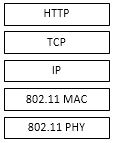
\includegraphics{intro/diagrams/tcpip.png}
	\caption{802.11 in the TCP/IP stack.}
\end{figure}

802.11 is split in to various task groups again which define extra amendments to the standard, the most prolific task groups are TGb, TGa, TGg and most recently TGn.

\begin{table}[htb!]
\begin{center}
	\begin{tabular}{| c | p{ 5cm } |}
		\hline
		\textbf{Task Group} & \textbf{Amendments} \\ \hline
		TGa & This amendment operates in the 5GHz band with a maximum data rate of 54Mbit/s, which allowed it to operate away from the noise of devices in the 2.4GHz band. This amendment is no longer valid. \\ \hline
		TGb & This is an amendment to the original standard, marketed as WiFi, which brings throughput up to 11Mbit/s, and was implemented worldwide. Products that supported this amendment started to appear during 1999, starting with the Apple iBook. \\ \hline
		TGg & TGg allows for 54Mbit/s throughput in the 2.4GHz band, the same throughput as TGb. \\ \hline
		TGn & Allows for multiple antennas to increase the maximum data rate, getting up to 600Mbit/s when usng four spatial streams at a 40MHz channel width. \\ 
		\hline
	\end{tabular}
\end{center}
\end{table}

\subsubsection{802.11 Key Terms}

The 802.11 specification defines a number of components that make up various network architectures \cite{intro:80211_lecture}, which shall be referenced through the document.

\subsubsection*{Station}
A device that has the ability to connect to the wireless access point using the 802.11 protocol. For example, a desktop PC, laptop, smart phone, etc. The specification formally defines a station as:

\begin{center}
\quote Any device that contains an IEEE 802.11-conformant medium access control (MAC) and physical layer (PHY) interface to the wireless medium (WM).
\end{center}

Station is often interchangeably referred to as a node or client and can be either fixed, or mobile.

\subsubsection*{Access Point}
Access points are, more often than not, dedicated hardware devices that act as the central receiver and transmitter of a wireless network. Some wireless adapters have the ability to act as soft access points, which is how, for example, smartphones are able to become hotspots for devices without an internet connection.

\subsubsection*{Base Service Set(Base Service Set)}
A BSS is a group of stations that are connected to an access point which is connected to a wired network.

\begin{figure}[htb!]

\centering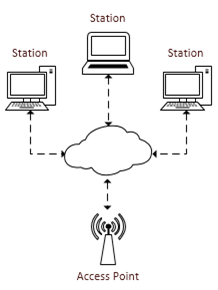
\includegraphics{intro/diagrams/bss.png}
\caption{An example BSS.}

\end{figure}
\newpage
\subsubsection*{Base Service Set Identification (BSSID)}
The unique identifier given to a BSS, in an infrastructure BSS this is the MAC address of the access point. In an ad hoc network (IBSS), with no governing access point, it is random and administered by the starting station \cite{intro:ieee_tutorial}.

\subsubsection*{Service Set Identification (SSID)}
The human readable  string given to a BSS, chosen by the access point, that is broadcasted in beacon and probe frames.
\newpage 
\begin{figure}[htb!]
\centering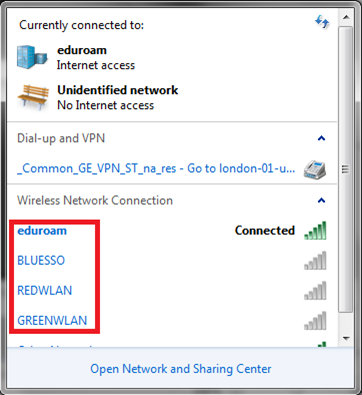
\includegraphics{intro/diagrams/ssid.png}
\caption{An SSID as displayed in Windows network manager.}
\end{figure}

\subsubsection*{Extended Service Set (ESS)}
An ESS is a group of two or more infrastructure BSS that share the same SSID and security credentials where the access points communicate to forward traffic and the movement of stations between the BSSs. This communication is performed by the distribution system (DS), which is out of the scope this report.

\begin{figure}[htb!]
\centering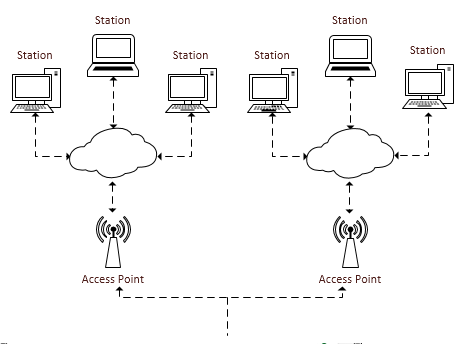
\includegraphics{intro/diagrams/ess.png}
\caption{Two BSS making an ESS.}
\end{figure}
\newpage

\subsubsection{802.11 Security}

The 802.11 is an inherently insecure \cite{intro:80211_lecture} base on which a large majority of enterprise applications are founded upon. Attempts have been made to secure networks by using various types of encryption, for example Wired Equivalent Policy (WEP) \cite{intro:netgear_wep} and WiFi Protected Access (WPA) \cite{intro:wiki_wpa}, however these standards only encrypt the data portion of the exchange. Management frames are left open and unencrypted which offers opportunity for exploitation in a number of ways- in which I go in to more detail in section \ref{sec:attacks}- from getting unsuspecting users to connect to a faked access point (page \pageref{sec:spoofap}) to collecting data based on access points a mobile device has connected to through the period beacon frames (page \pageref{sec:honeypot}).
 
\subsubsection{Leaky Applications}

There have been reports recently \cite{intro:bbc_flashlight_app} of applications written for Android that have been collecting and sending data to advertisers, from what is perceived as innocuous information such as phone model and screen size, to personal data including, but not limited to, current location information, gender and date of birth, then at the extreme end entire contact lists. It has come to light, from the documents leaked by Edward Snowden, that GCHQ and the NSA have been targeting apps that send this type of data, unencrypted, back to advertisers as it allows them to build a profile of the user. This profile can be built using similar methods to the Evercookie, that works on the premise of collecting as much information as it can about the user and hashing this so that it gives a unique identifier for the user. Methods such as this have proven effective when attempting to circumvent UK cookie laws, by tracking users through fingerprinting methods.

\subsubsection{Profiling Users}

Fingerprinting is achieved by collecting as much information as you can about the user through commonly available methods, and then hashing the data and storing it either in a local database- or through a persistent cookie such as the Evercookie \cite{intro:evercookie}. It has been noted that if a user has Flash and Java enabled, the success rate of uniquely identifying is 94\% \cite{intro:unique_browser}. 

Interestingly, a paper \cite{intro:twitter_home_location} came out recently that documented the process they took in identifying the geo-location of Twitter users that did not include geotags by comparing the information in the content, hashtags, foursquare check-ins, locational references, etc. to those that had geotags in them. They found that, when omitting users identified as travelling, they could predict the home location from tweets to 68\% for cities, 70\% for states, 80\% for time-zones and 73\% for regions. This style of data mining highlights the effect that other users sharing personal location information can have on those that chose to omit the data. 

One of the golden nuggets [NSA] of unencrypted data is a photo upload, ideally to social media, but any endpoint will do. The reason for this is the Exif data that accompanies the photograph. This can detail various pieces of information on modern smartphones with a GPS chip, but most importantly it contains the make and model, datetime stamp and GPS location (geotag). These fields are often added by default. 

[Picture from Exif app of extracted data]

Social media websites, such as Facebook and Twitter, strip any Exif data from uploaded photos in an attempt to preserve the privacy of their users. This can be effective at stopping their users from taking data from photos; however, depending on when during the upload process this takes place it is still susceptible to wiretapping (referring here to both a MITM attack and by public entities at locations they would have access to \cite{intro:room_641a}) if the user is not transmitting over HTTPS. Wiretapping in this instance can refer to either a higher body monitoring traffic, or a malicious user performing a man in the middle attack on the wireless network. If, for example, the photo is sanitized on the client side, this means that Exif data is not transmitted and is not susceptible to wiretapping; however, if this action is performed server side then the Exif data is transmitted and is open to monitoring. There is an argument brewing in creative industries that stripping the Exif data destroys any copyright information the picture may be able to carry as they often manage this data to allow them to detect when their image is being used without their permission.

There has been a recent shift to move to forcing HTTPS by default on websites as a way of deterring Joe Bloggs from attempting attacks on open encrypted networks. It encrypts any traffic to and from the client using SSL, and prevents MITM attacks, although if HTTPS is only used during the login stage of a website to gain access, and then reverts back to HTTP and sends session data, the session can still be hijacked.

Angry Birds hit the headlines when it was named in one of the NSA/GCHQ releases as an application they can exploit to gain user data. Being an incredibly popular game, it demonstrates the ease in which users can be coerced into allowing applications access to their data.

\subsubsection{Culmination}

This project takes inspiration from the information detailed above. It sets out to develop an application that analyses probe request frames and sends spoofed probe response frames in order to establish itself as an access point for any unencrypted requests. This application will then display HTTP packets, demonstrating how smartphones have an inherent security vulnerability with their preferred network lists. Alongside this an Android game will be developed that intentionally leaks personal and location data unencrypted across the network. This will then be combined with the first application to demonstrate how apps can broadcast your personal data, unknowing to you, to an attacker as you pass by. It would be preferable to develop an application that extends the first, graphically displaying profiles built through leaked data collected.

\subsection{Objectives}
This aim of this project to expose the inherent security vulnerability that unencrypted and WEP encrypted networks leave behind on mobile wireless devices whilst they pass by in the pocket of the owner. This will be achieved by developing software capable of responding to 802.11 probe request frames emitted by roaming smartphones in an attempt to masquerade as the requested access point.

Once a connection with a device has been established the laptop running the software will create a bridge between the soft access point and the hardware to allow for traffic to pass normally, and HTTP traffic to be analysed. The security vulnerabilities will be demonstrated by an Android game, similar to one in the top charts currently, that has been written with the sole intention of leaking data. 

Finally, I want to look into what steps can be taken to prevent this attack happening at root level, and the possible ways of adding security at application level to notify users of hijacking attempts.

\subsection{Content}
There isn't any.
\clearpage
\section{RESEARCH}
\clearpage
\subsection{Attack Vectors}
There are a number of attacks that take advantage of insecurities in the 802.11 standard and that capitalize on unencrypted or WEP encrypted networks.  Where the attacks were demonstrated, they were performed using a laptop running BackTrack running in a virtual machine, with an Alfa wireless adaptor.

The attacks that I have documented all lend themselves to the overall application I am trying to implement, either by complimenting or directly using tools, applications and principles that will come in use.

\subsubsection{Spoof Access Point}
\label{sec:spoofap}
This is not necessarily an attack in itself, but a means of relying on social engineering to gain connections to perform attacks on. A soft access point is a rogue access point that has been established on a wireless adaptor, without the need for a router. Leaving this open, and performing in an area with a high footfall, or cafe area, for example, will allow the attacker to gain connections, monitor traffic, and perform various man-in-the-middle attacks. It can also be paired with other attacks detailed further on in the report.

\begin{figure}[h!]
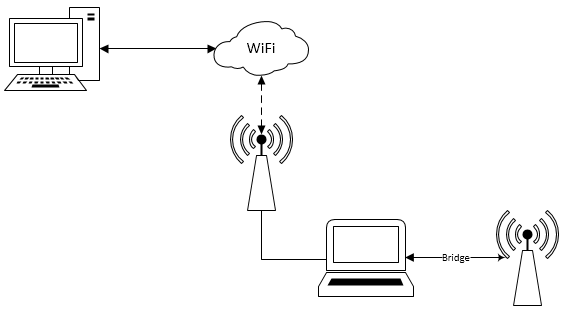
\includegraphics[width=\linewidth]{research/figures/spoofap.png}
\caption{Soft access point bridges traffic to real access point.}
\end{figure}

\subsubsection*{Performing the Attack}
As this is more of a gateway attack, not a lot can be gained from doing it alone. The airbase-ng tool proved the simplest way to create a fake access point, taking the wireless interface and either start or stop as parameters. The image below shows the creation of an access point and a station connecting to it.

\begin{figure}[h!]
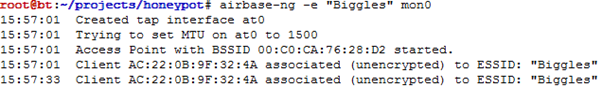
\includegraphics[width=\linewidth]{research/attackvectors/figures/spoofap1.png}
\caption{Soft access point created with the SSID “Biggles”.}
\end{figure}
\subsubsection{Man in the Middle (MITM)}
The man in the middle attack puts the attacker between the station and the access point, allowing them to eavesdrop on communications taking place. In wireless communications, monitoring passing traffic is trivial considering traffic is broadcast and picked up by all network cards in the vicinity; but usually discarded if not intended recipient. This attack allows the attacker easy access to user data sent over unencrypted protocols such as HTTP, but also allows them to use tools such as sslstrip \cite{research:ssl_strip} to attempt to thwart HTTPS.

\begin{figure}[h!]
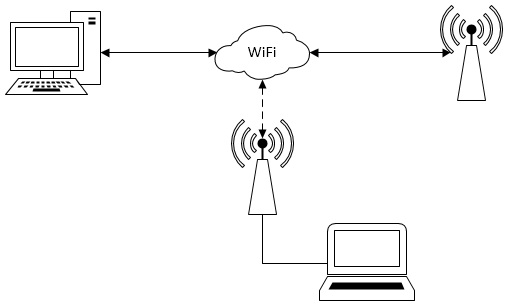
\includegraphics[width=\linewidth]{research/figures/mitm.png}
\caption{Malicious user monitors and injects data packets in to traffic.}
\end{figure}

This style of attack is a popular choice when communications involve some type of public key encryption. 

A more recent variation to this attack, that reflects the shift toward web applications, is the Man in the Browser\footnote{The Boy in the Browser attack \cite{research:bitb} is a less mature version of the Man in the Browser attack. It is a trojan that routes traffic to the attacker’s proxy website to modify before sending to the intended destination.} (MitB). The advantage this has over the vanilla MITM attack is SSL style authentication measures do not hinder its effectiveness. Examples of the MitB attack include HTTP Cache Poisoning \cite{research:cache_poisoning} and HTTP Response Splitting \cite{research:response_splitting}, both can leave lasting effects on the compromised browser.

%This attack will feature in the project implementation as a means of inspecting leaked data from applications when stations are caught in the honeypot.
\subsubsection{Deauthentication Denial of Service}
\label{ddos-atk}
The deauthentication denial of service (DOS) \cite{research:disassoc_atk} is a complex attack that takes advantage of the unencrypted nature of the management frames by spoofing disassociation or deauthentication frames, depending on whether the attacker wants to block a single device or all devices from the network. It is a denial of service attack that targets the MAC layer in the TCP/IP Model pictured in figure \ref{tcpip}, there are other attacks designed for the other layers \cite{research:layer_flood}.

When a client wishes to gracefully disconnect from a 802.11 network it sends a disassociation frame \cite{research:80211_disassoc_frame} to the access point, likewise when an AP needs to disconnect from a client it sends a deauthentication \cite{research:80211_deauth_frame} frame. If the AP needs to disconnect all clients, e.g. in the event of a reboot, it broadcasts the disassociation frame. 

The unencrypted nature of these frames leaves them open to MAC address spoofing of either the client or access point, meaning an attacker can forge frames from either source. It has been noted that deauthentication frames are preferable to spoof due to the access point and client having to perform the entire authentication cycle again in order to carry on using the network \cite{research:defending_auth}.

\begin{figure}[htbp!]
\centering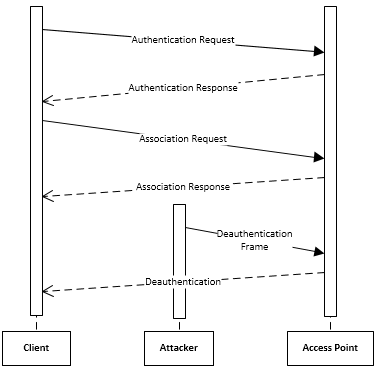
\includegraphics{research/attackvectors/figures/ddos.png}
\caption{Deauthentication DOS sequence.}
\end{figure}

The beauty of the deauthentication DOS is that it can be launched from relatively inexpensive hardware, as demonstrated with the Alfa, when paired with a good technical knowledge- especially when using a pre-support applications \cite{research:aircrack}. It should also be noted that this attack may not be started with malicious intent, as, for example, you have a network with a hidden SSID that users have discovered and hijacked, you can use this to deauthenticate all the stations to recover the network. On the more malicious side, this attack can be used to force users to connect to a spoofed access point after performing this attack, then chaining on a MITM attack. 

Chaining this attack with a spoofed access point, and then performing a MITM is an example of an advanced attack that could be performed on unknowing users in a public location. Utilizing beacon frames to start the chain of attack leaves security software that tracks spoofed MAC addresses completely useless. You can determine the MAC address of the real access point by monitoring beacon frames and taking the value set as the source address, then using it source in the deauthentication DOS, and then subsequently the spoofed access point setup.

\subsubsection*{Performing the Attack}
To gain a better understanding of this advanced attack I performed it on myself and documented the results. I set up my wireless router to broadcast an open network, laptop running BackTrack, tablet connected to the wireless network, and wireless adaptor in monitor mode.

\subsubsection*{Discovering the Access Point}
Although I knew the SSID and could get the MAC address of the access point I would be targeting, I wanted to perform it from the perspective of somebody that didn't, and needed to circumvent security software. In order to achieve this first step I decided to use the airomon-ng tool. This tool monitors beacon and probe request frames broadcast within range, and prints the MAC address of the source, and the SSID of the station. Figure \ref{ddos-1} shows the output of this application, and reveals the MAC address of the access point, ``Biggles'', I am targetting.

\begin{figure}[h!]
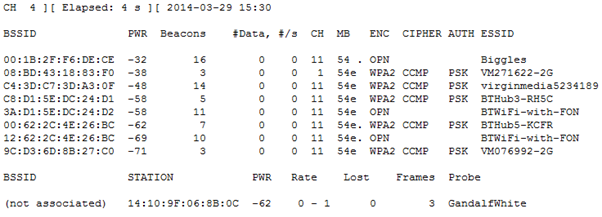
\includegraphics[width=\linewidth]{research/attackvectors/figures/ddos-1.png}
\caption{List of AP SSIDs in range of the wireless antenna.}
\label{ddos-1}
\end{figure}

\subsubsection*{Sending the Deauthentication Frame}
As the access point is transmitting on channel 11, I needed to either switch it to the same channel as the wireless adaptor monitor interface, or switch the monitor interface to channel 11. Again, as this was from the perspective of an attacker, I opted to switch the monitor interface channel as would be done in the field. After the channel change I could use aireplay-ng [8] to send a number of deauthentication frames with the spoofed MAC source and destination addresses, which is shown in figure \ref{ddos-3}.

\begin{figure}[h!]
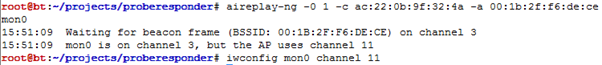
\includegraphics[width=\linewidth]{research/attackvectors/figures/ddos-2.png}
\caption{Changing the interface's channel.}
\end{figure}

\begin{figure}[h!]
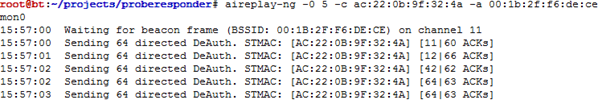
\includegraphics[width=\linewidth]{research/attackvectors/figures/ddos-3.png}
\caption{Sending the deauthentication frame.}
\label{ddos-3}
\end{figure}

\begin{figure}[h!]

\includegraphics[width=\linewidth]{research/attackvectors/figures/ddos-4.png}
\caption{Nexus 7 disassociating with the Netgear wireless router.}
\end{figure}

\subsubsection*{Introducing the Evil Twin}
To take this attack one step further toward the advanced chain of attacks, I created a fake access point that was making use of the Alfa wireless adaptor's ability to broadcast at a stronger signal than the access point. Figure \ref{ddos-5} shows the device connecting to the Evil Twin and leaving it open to any malicious intent I had.

\begin{figure}[h!]
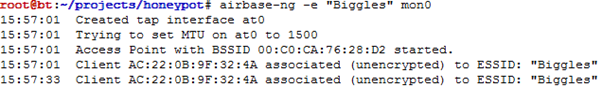
\includegraphics[width=\linewidth]{research/attackvectors/figures/ddos-5.png}
\caption{Station associating with the fake access point.}
\label{ddos-5}
\end{figure}
\clearpage
\subsubsection{Evil Twin/Honeypot Attack}
\label{sec:honeypot}
The Evil Twin, aka Honeypot, WiFi Phishing, AP Phishing, etc., is a gateway attack leveraged to give the attacker the ability to perform other exploits. Victims leave themselves open to a whole host of MITM exploits, including HTTP cache poisoning and DNS poisoning, along with having secure information such as credit card information, website login credentials and personal data stolen. Particularly worrying is the coupling of a honeypot attack, and then a MITM attack that includes the use of SSLstrip [3][5] in an attempt to beat HTTPS. There are new protocols that have been proposed that would prevent this, such as HTTP Strict Transport Security (HSTS) [4]; however, this is out of scope of this project.

The attack takes advantage of the Preferred Network List (PNL) that wireless devices maintain once successful connection with an access point has been made. When a device is not connected to a wireless network, it will broadcast probe request frames of all the previous networks it has been attached to. When attached to a network, it broadcasts probe requests for that network to allow it to roam between BSSs in an ESS. 

\begin{figure}[h!]
\centering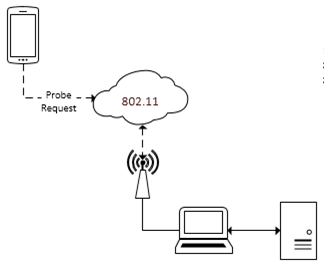
\includegraphics{research/attackvectors/figures/honeypot.png}
\caption{The smartphone sends a probe request frame which is picked up by the attacker.}
\end{figure}

The attack can be traced as far back as 2003 [0], with the KARMA Wireless Client Security Assessment Tools [1] arriving in 2005 and making it even more accessible by releasing patches for the Linux MadWifi driver, allowing applications to create fake 802.11 access points in response to probe request frames from 802.11 capable devices. This application was released purely as a gateway to users writing their own exploits, termed BYOX (Bring Your Own eXploit). This set of tools was certainly ahead of its time in the security landscape, as wireless enabled devices were scarce when compared to today where not only smartphones are increasingly popular [6], but with the advent of The Internet of Things, and the preference to use WiFi in products [7][8][9], more devices are being made vulnerable to old attacks.  

To perform the attack, the attacker needs to gain the SSID of access points either through beacon packets of real access points if performing a disassociation evil twin attack, or by probe requests broadcast by passing devices if performing the honeypot style. If a real access point is found the attacker can disconnect users from the real AP through a deauthentication DOS and broadcast the fake AP beacon packets with a stronger signal than the real one. Passing devices sending out probe requests will connect to the AP with the strongest signal, which happens to be the fake one. If the attacker is sniffing for probe request frames to perform a honeypot, all they need do is perform the association sequence once a valid probe request frame is detected. This can be achieved using low-level packet injection/monitoring libraries, or through a suite of tools common to penetration testing distributions.  

This attack is not thwarted by Wired Equivalent Privacy (WEP) or WiFi Protected Access (WPA) as they only encrypt data after the association is established, thus not protecting against management packet spoofing [1]. There have been efforts made to protect against this attack, not by protecting against MAC spoofing, but by utilising the received signal strength (RSS). This proves a good method of protection for single transmitter source, but it has also been demonstrated to have a 97.8\% success rate with multiple transmitters [3]. 802.11w does implement protected management frames and as a result would eliminate this style of attack, I touch upon this in section \ref{80211w}.

The honeypot attack forms the basis of the program this project is implementing and as such will be detailed in the implementation section of the report.
\subsection{Low-Level Libraries}
\subsubsection{libpcap}
libpcap was developed by the Network Research Group at Lawrence Berkeley Laboratory, it is the low-level packet capturing code from tcpdump taken and put in to a library.  
\subsubsection{LORCON}
LORCON is an open source 802.11 frame monitoring and injection library that sets out to abstract the driver specific functionality required to allow the developer to easily develop network penetration applications. It came into being after it was identified that when writing tools it required a rewrite each time raw transmission was figured out for a new driver.

It completely abstracts any driver level interaction by allowing the developer to call functions such as:

\begin{verbatim}
driver = lorcon_auto_driver(interface);
context = lorcon_create(interface, driver);
lorcon_open_inject(context);
\end{verbatim}

Which is all that is required to set a driver in to injection/monitor mode- assuming it is supported.

Similar to libpcap- due to LORCON using libpcap- you can then pass a callback to the lorcon loop which will be called each time a packet is received.

\begin{verbatim}
lorcon_loop(context, count, callback, NULL);
\end{verbatim}

Packets are parsed once received and all data is easily accessable through defined structures. It also includes extra information for 802.11 frames that it captures, which makes it ideal for the the capture and injecting part of the honeypot application. For example, to determine whether the packet we've captured is of a certain type we're interested on we can simply switch on:
\begin{verbatim}
 *extra = packet->extra_info;

 switch(extra->type) {
 	case 80211_MNGMNT:
 		 switch(extra->subtype) {
 		 	case 80211_PROBE_REQ:
 ...snip...
\end{verbatim}
Lorcon is able to run on BackTrack and Kali, meaning that it can be used on Kali's ARM distribution with a little modification of the build process. This is out of the scope of the main project; however, will be considered in the conclusion. It also has bindings available in Ruby (ruby-lorcon) and Python (PyLorcon2) that are useful for rapid prototyping and testing wireless chipsets to determine whether they are compatible.

%\begin{verbatim}
%[1] http://en.wikipedia.org/wiki/Lorcon
%[2] http://packetfactory.openwall.net/projects/libradiate/802.11_toolkit-2.0.pdf
%\end{verbatim}
\subsection{Hardware}
The selection of hardware for usage in this product comes down to a combination of two vendors. Firstly the wireless adaptor manufacturer, such as Edimax, Netgear, Belkin, etc. that build the overall product. The decision of which manufacturer in this respect is not as important as the second, the chipset manufacturer.  These are companies such as Broadcom and Realtek, and this decision determines which operating systems are compatible, the device driver to use, and ultimately whether injection and monitoring are supported.

\subsubsection{Wireless Adaptor}
This boils down to device type, i.e. whether the adaptor is PCI, USB, etc. and does not make any particular difference.
\subsubsection{Wireless Chipsets}
Consideration has to be taken into the chipset wireless adaptors use for compatibility with injection and monitoring libraries. Certain vendors, such as RealTek, support the open source community more-so than others which means drivers can be written for adaptors that use them.

Firstly I tried to use a wireless adaptor purchased for use with the Raspberry Pi. 

\begin{figure}[h!]
\centering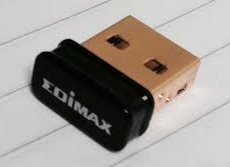
\includegraphics{research/figures/edimax.png}
\caption{Edimax EW-7811UN wireless adaptor.}
\end{figure}

The Edimax EW-7811UN fulfilled the first part of the criteria by using the RTL8188CUS chipset as working drivers were available for Linux; however, after initial tests against PyLorcon2 it was determined that the adaptor was not supported. Most likely due to it's newer chipset and Lorcon having not been updated in approximately two years. 

The second suggestion for a wireless adaptor to use with Lorcon was the Alfa AWUS036H, which came from various support forums that had users querying which adaptor to use with the Air-ng applications.  

\begin{figure}[h!]
\centering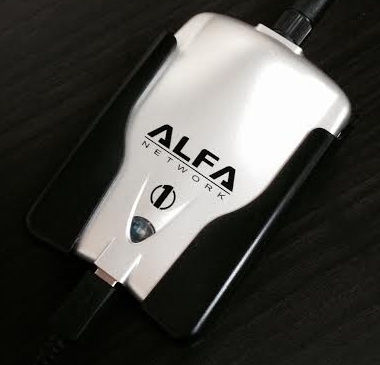
\includegraphics{research/figures/alfa.png}
\caption{Alfa AWUS036H wireless adaptor.}
\end{figure}
\newpage
This is ideal as that suite of software will more than likely play a large role in the application's implementation as it is very good at specific tasks such as creating fake access points, and creating wireless monitor mode interfaces. The Alfa wireless adaptor is built upon the Realtek RTL8187 chipset, which, as noted above, is also beneficial due to RealTek's support toward the open source community.
\subsection{Operating Systems}
There are two ideal Linux distributions that have been developed with the purpose of being used for network penetration testing and have various applications and tools pre-installed to take advantage of WiFi vulnerabilities. One of these distributions also has a version compiled for ARM that will allow the software to run on embedded platforms, with little porting, such as the IGEP V2 and cheaper alternatives, the Beagleboard and Raspberry Pi.

 I have tested each of the distributions, firstly to determine whether the Air-ng applications would install and run, as if they wouldn’t it was almost a guarantee that programs written using Lorcon would not work correctly, then once it was determined these would run, I tested a couple of wireless adaptors by setting up a soft AP, bridging this the actual hard AP, and forwarding traffic through it, using the Air-ng suite, as this would produce a similar effect to the final application.

\subsubsection{Backtrack 5 R3}
Backtrack was a security distribution that focused digital forensics and penetration testing. It comes pre-installed with a whole host of applications and tools, and was bootable from Live CD and USB. 

This distribution comes with the Air-ng applications pre-installed, which was a good guarantee that any attempts to use libraries based on libpcap will meet little resistance from install.

Backtrack is unfortunately no longer supported; however, a branch- Kali Linux- has been developed and is actively updated.
\subsubsection{Kali}
Kali marked the switch from an Ubuntu base to Debian for the Backtrack developers. One of the big updates from Backtrack is further support for ARM devices, which means it can be run on the Raspberry Pi. This is a huge benefit as it would reduce any effort in porting the application to an OS running on the board.


\clearpage
\section{Requirements}
This requirement specification uses keywords to indicate requirement levels as defined in RFC 2119 \cite{req:rfc_must}. Consideration has been taken to follow principles outlined in the IEEE Recommended Practice for Software Requirements Specification \cite{req:ieee_spec}, whilst being mindful that they are included as part of a larger document.

\subsection{Scope}
The requirements set forth are for the Honeypot application that will be used to create spoofed access points based on probe request frames broadcast from passing mobile wireless devices, the Android application that leaks personal data, and server. The requirements are split into separate sections that define the hardware and software requirements for the honeypot application, then moves on to define the specific requirements for the honeypot application itself, the leaky Android application and simple server application.

\subsection{Overall Requirements}
\subsubsection{User Interfaces}
The honeypot application will have no graphical user interface (GUI) and will provide relevant, contextual, information to the user through a simple console interface. Relevant information is defined below as part of the functional requirements. Usage of the application will require some prior knowledge of the 802.11 standard and its naming conventions.

Messages displayed to the user may be configurable in terms of debug, information, warning and error. Notification of the desired level should be configurable while starting the application, but not during application execution.

Viewing of TCP data may be performed by an external application, such as Wireshark. Using such an application will require previous experience of creating filters to find the desired traffic.

\subsubsection{Hardware Interfaces}
Due to the application needing to be run in a high traffic area, to make it as effective as possible, it will need to be executed on a laptop. The Operating System may either installed as the primary, or, run in a Virtual Machine.

The honeypot application requires a wireless adaptor that conforms to the standards determined in section \ref{research:hardware}. To summise, they are as follows: possesses the ability to be put into monitor mode to capture traffic on the network, support for packet injection into the network, and support from the chipset manufacturer toward the open source community, as this will give us greater confidence in the drivers for Linux supporting the capabilities required, and working out-of-the-box.

Considering these points, and having used it during the research portion of this project, the Alfa AWUS036H (pictured in figure \ref{research:fig-alfa} on page \pageref{research:fig-alfa}) has been selected as the wireless adaptor.

A laptop will be required to run the application, and it will need at least one spare USB port for the wireless adaptor to be plugged in to and a spare ethernet port to connect to a wireless router.

The wireless network must have the SSID hidden, must have no encryption and must be connected to the laptop via ethernet cable. This is required so that the spoofed AP may bridge its traffic and the users of the spoofed AP will be able to access the internet

\subsubsection{Software Interfaces}
The application must run on Backtrack 5 Revision 3 (B5R3). The application may run on Kali Linux which is a derivative of Backtrack developed by the same team.

The Operating System must be either installed as the primary, or installed on a Virtual Machine. If the Operating System is installed on a Virtual Machine then the virtualisation software used must be VirtualBox V4.3.0. The network adapter in VirtualBox must be set to bridged and utilize the ethernet adapter of the host laptop.

Air-ng may be utilized to create the spoof access point once the requirements of the AP have been determined. This software suite comes pre-installed on the required Operating System. 

\subsubsection{Communications Interface}
As this application is designed to exploit vulnerabilities in the 802.11 standard, 802.11 will be required as a protocol. At the higher level TCP traffic data will be analysed for information.

\subsubsection{Operations}
Once the application has been started by the user it must be entirely autonomous, acting upon user defined parameters at execution. The only user interaction should be exiting the application, which on signal it shall gracefully exit.

\subsubsection{Site Adaptation Requirements}
This application must only be run only in controlled wireless lab conditions due to the inability to get informed consent of the participants when running publicly. Under no circumstances should the application be executed in a public location, without a predefined SSID filter.

The application will require the host machine to be connected to an internet source via ethernet in order for it to successfully bridge traffic.

\subsubsection{Constraints}
The application will not be able to perform the honeypot attack on mobile devices that broadcast probe requests for encrypted networks. It will also be limited to the Operating System in which it has been developed to run on, in this instance that is Backtrack 5 Revision 3 or Kali. The application will only support one fake access point at a time due to the limitations imposed in order to meet ethical guidelines.

\subsubsection{Assumptions}
It is assumed that the Operating System running on the Virtual Machine will have access to the network that the host machine is connected to, and this will be connected via Ethernet.

\subsection{Specific Requirements}
This section justifies the requirements and lists them with a numerical value in order to track them through the design, implementation, and testing stages.

\label{requirements:specific}
\subsubsection{Honey Pot Application}
\begin{enumerate}
\item Take user defined parameters

The application shall accept an SSID to filter the received probe request frames to ensure that data capturing is limited to devices owned by the user testing the application, but still allow testing of multiple devices at a time. It must also accept the wireless interface that the application is to act upon.

\item Filter packets based on SSID

As explained prior to this, filtering enables the application to run in an ethically sound way.

\item Capture and parse probe request frames

The probe requests are the gateway to identifying vulnerable devices.

\item Allow device to connect to spoof access point

Once a device has been identified as vulnerable the application must spawn a fake access point using credentials found in the probe requests broadcast. This may either be implemented programmatically, or by take advantage of existing solutions.

\item Send probe requests captured to the server

The server may be capable of profiling passing device owners through SSIDs broadcast, so the honeypot application must support sending the MAC address and SSID of each probe request to the server using TCP.

\item Determine authentication type of previous network

To cut down on the number of wasted attempts at hijacking device traffic, the honeypot application must predetermine whether the device is searching for a network with open authentication.

\item  Bridge traffic from the mobile device

In order for the device to access the internet, and for the attacker to capture data packets, the fake access point must have their traffic bridged to an actual network with internet access.
\end{enumerate}
%%%%%%%%%%%%%%%%%%%%%%%%%%%%%%
\subsubsection{Android Application}
\begin{enumerate}
\item  Emulate a popular Android application

To demonstrate how easy it is for seemingly harmless applications to access and send personal data, the application must be similar to a currently popular application.

\item  Capture the users location data

As detailed in section \ref{intro:leaked-data} applications are increasingly sending information to advertisers in order to deliver personalised content. Location data is popular as it allows advertisers to deliver location-based advertisements, so, to mimic this, the application must report the device's current location. 

\item   Capture a unique identifier for the device

Future expansion may allow the server to profile unique devices. In order to facilitate this, the application must send a unique identifier with each message.

\item  Send the captured data to the server with no encryption

The application must send the data unencrypted as the whole reasoning behind this is to demonstrate an application that leaks data.
\end{enumerate}
%%%%%%%%%%%%%%%%%%%%%%%%%%%%%%
\subsubsection{TCP Server}
\begin{enumerate}
\item Accept a number of clients connecting and disconnecting

To support the application's implementation of a TCP client, and multiple devices, the server must be able to handle multiple connections and disconnections.

\item Display the packets received

The server must print each packet received in a user friendly manner.
\end{enumerate}
\clearpage
\section{Design}
\subsection{Design Overview}
The design is split into a number of sections.Firstly I detail the software components that make up the overall system. Then I go in to detail more detail on each component. We start with the Honeypot application that finds and attacks vulnerable devices, and then move on to looking at the structure of the leaky Android application and how to overcome the problem of using platform specific code within the game, then look at the server application. 
\subsection{Overall System Architecture}
The scenario that this project hypothetically aims to work in is in an area with high traffic, such as a Student Union bar, or a busy public transport station. In reality the applications are designed to meet the ethical guidelines set forth at the beginning of the project whereby a user's consent must be gained prior to taking place in any experimentation. Due to this restriction care must be taken within the design to ensure, where appropriate, devices are filtered and ignored on a set of criteria. This criteria may be MAC address of devices broadcasting probe requests or the SSID present in probe requests. As set out in the requirements the filter will be based on the latter of the two proposed, filtering devices based on the SSID they are probing for. In doing so removes the limitation of testing one device at a time- theoretically having to update the MAC address filter for each new device- and allows us to connect multiple devices running different operating systems at the same time to determine the effectiveness of the overall implementation of the honeypot attack. It should be noted that the leaky application, designed to demonstrate the ease in which applications can broadcast personal data unencrypted, will only be available on Android due to the relative simplicity in creating an application for the environment, and availability of devices. 

\begin{figure}[h!]
\centering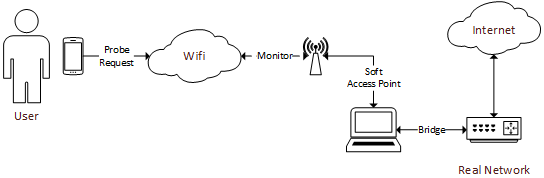
\includegraphics[width=\linewidth]{design/figures/overall.png}
\caption{Overall system architecture.}
\end{figure}

A soft access point is created on the detection of a valid probe request, which is defined as being a request from a device that is looking to reconnect to a network with no authentication method, and the network traffic is then bridged to an actual network to ensure that the user is still able to access the internet, and the attacker can monitor passing traffic.

\subsection{Honeypot}
\subsubsection{High Level Program Flow}
\label{program-flow}
Figure \ref{fig:honeypot_flow} details the high level application flow for the honeypot program. 

\begin{figure}[h!]
\centering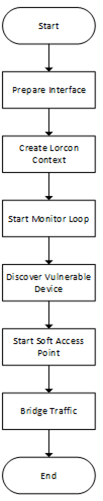
\includegraphics{design/figures/honeypot-flow.png}
\caption{Overall system flow.}
\label{fig:honeypot_flow}
\end{figure}

The application needs to start by creating an interface that is able to capture and inject packets, as this is required by Lorcon to create the context for the packet capture loop. Once setup the monitor loop can begin to parse captured packets until it finds a vulnerable device, after which the application spawns a fake access point and bridges the traffic.
\newpage
\subsubsection{Parsing Probe Request Frames}
\label{parsing-probe}
One of the requirements is to ensure that the SSID that the application looks for can be defined by the user. This argument defined on the command line is then taken by the application and used when parsing probe request frames, as detailed in figure \ref{fig:ssid-machine}

\begin{figure}[h!]
\centering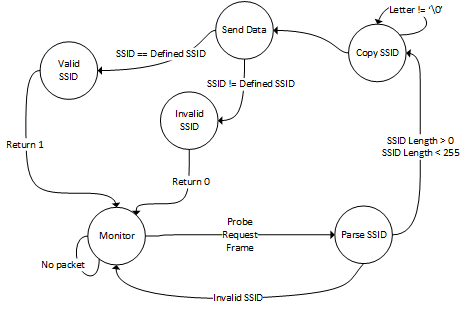
\includegraphics{design/figures/valid-ssid.png}
\caption{Probe request frame parser state machine.}
\label{fig:ssid-machine}
\end{figure}

The application firstly needs to find out whether the SSID is hidden, by checking if the length field in the header is 0, or invalid, by checking if the same field is greater than 255. If it is a valid SSID, it copies the SSID value from the packet header and compares it against the defined SSID from the user, then returns a value to the monitor loop. Also included is the TCP client sending data to the server each time it receives a valid SSID. 

\subsubsection{Discovering Vulnerable Devices}
\label{open-auth}
Figure \ref{fig:discover_device_seq} details the process in which the application goes through to discover a vulnerable device. It parses frame types until it finds a probe request, parses that request as defined in section \ref{parsing-probe}, then sending a response to trigger an association request from the device so it can determine the authentication type that the previous access point used. If it was an open access point that the device had previously connected to it returns a success value and allows the application to move on to the next  stage of the attack, creating the fake access point.
\clearpage
\begin{figure}[h!]
\centering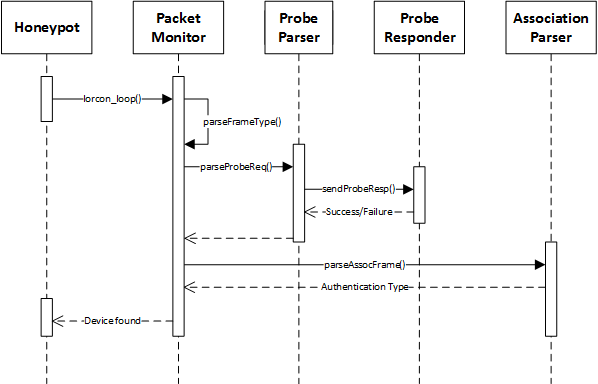
\includegraphics[width=\linewidth]{design/figures/discover-device-seq.png}
\caption{Discovering vulnerable device sequence.}
\label{fig:discover_device_seq}
\end{figure}

\subsubsection{Creating a Fake Access Point}
\label{design:create-ap}
The fake access point shall be created by forking the application and running Airbase-ng, as this is the quickest and most reliable way to achieve what is needed. Writing my own access point, whilst interesting, is not the goal of this project. Using Airbase to create a fake access point is covered in section \ref{sec:spoofap} on page \pageref{sec:spoofap}.


\subsubsection{TCP Client}
\label{hp-tcp}
As the honeypot application is required to collect data about probe requests being broadcasted, a simple TCP client is required to send data to the server. The data to be captured is as follows:

\begin{enumerate}
\item MAC address of the device
\item SSID the device is looking for
\end{enumerate}

Due to the simple nature of this the application will concatenate the two string values using a delimiter to enable the server to easily tokenise and parse the message. In this case I have opted to use a comma as the delimiter, giving the message this structure:

\begin{verbatim}
00:de:ad:00:be:ef,Wireless Lab
\end{verbatim}

As we cannot guarentee the server will be active at all times, the client must connect and disconnect each time it attempts to send data, as detailed in figure \ref{fig:hp_tcp_server}. 

\begin{figure}[h!]
\centering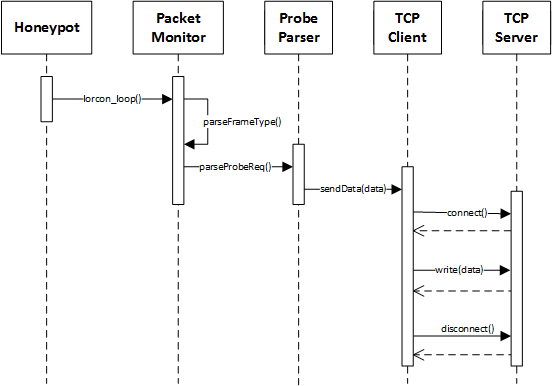
\includegraphics[width=\linewidth]{design/figures/hp-tcp-client.png}
\caption{TCP client/server interaction.}
\label{fig:hp_tcp_server}
\end{figure}

\clearpage
\subsection{Android Game}
\subsubsection{Flappy Bird}
\label{design:flappy-bird}
I have chosen to clone a recently popular game, that has seen an increase of clones in the past few months, Flappy Bird. The reason for chosing this is the simplicity of the overall game, and the virality that it has displayed. This version will be named Leaky Bird to reflect it's actual purpose of leaking data, not being fun. 

\begin{figure}[h!]
\centering
\includegraphics{design/figures/flappy-b-1.png}
\caption{Flappy Bird's simple instructions.}
\label{fig:android_fb1}
\end{figure}

The premise behind Flappy Bird is simple, the player needs to tap the screen in order to make the bird rise and go through a pair of gates, in the form of pipes. Each time the player successfully maneuvers through a set of obstacles the player is awarded a point.

The total points are recorded, and the top three recorded in the high scores. The artwork from the game was borrowed from a well known game publisher, Nintendo, who used similar sprites in their Mario titles.

\subsubsection{Leaky Bird Sprite Sheet}
As the game is not the main focus of this report, and is a clone of an existing game, a sprite sheet will be used that consists of the original artwork, pictured in figure \ref{fig:leaky-spritesheet} on page \pageref{fig:leaky-spritesheet} in the Appendix. This spritesheet will be split in to separate images by the game.

\clearpage
\subsubsection{Leaky Bird Class Diagram}
The Leaky Bird game design, similar to it's parent game,  is relatively simple. It consists of two main classes that inherit from the libgdx screen class, with the GameScreen class holding the GameRenderer and GameWorld which renders and holds the game state respectively doing the majority of the work.

\begin{figure}[h!]
\centering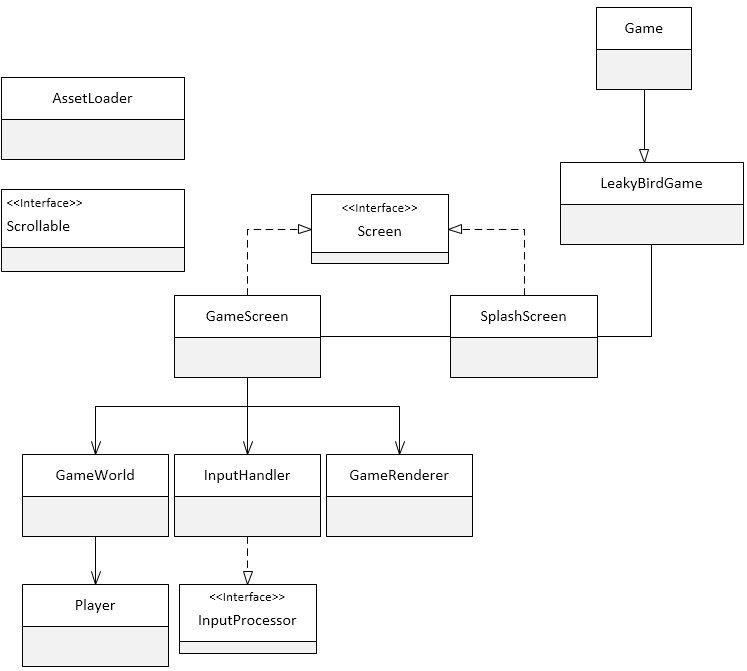
\includegraphics[width=\linewidth]{design/figures/ag-cd.png}
\caption{Android game class diagram.}
\end{figure}
\clearpage
\subsubsection{Android Location Provider}
\label{design:ag-lp-cd}
To successfully use platform specific functionality within the libgdx game environment an interface needs to be created to allow use of the functions. More detail on this can be found in the implementation section; however, figure \ref{alp-class} details the classes required to provide the game with the ability to get location information from the Android device.

\begin{figure}[h!]
\centering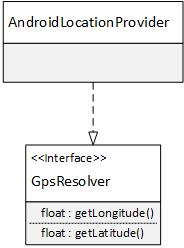
\includegraphics{design/figures/ag-lp-cd.png}
\caption{Android Location Provider class.}
\label{alp-class}
\end{figure}

\subsubsection{TCP Client Provider}
\label{design:ag-tcp-1}
Android applications require any network communications to be performed on a separate thread to that which the UI is currently running on. This stops the application from becoming unresponsive during long connection times or heavy data transfers. As a result of this the TCP client connection, data transfer, and disconnection must run on an AsyncTask when executed otherwise the application will throw an android.os.NetworkOnMainThreadException, so this requires another interface to be written to encapsulate the Android specific library. 

\begin{figure}[h!]
\centering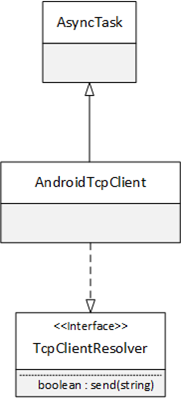
\includegraphics{design/figures/tcp-cd.png}
\caption{Android TCP client class diagram.}
\end{figure}

Similar to the GpsResolver class, the Android MainActivity will pass through an AndroidTcpClient that implements the TcpClientResolver interface for the game to make of use of when it needs to transmit data to to the server.

\begin{figure}[h!]
\centering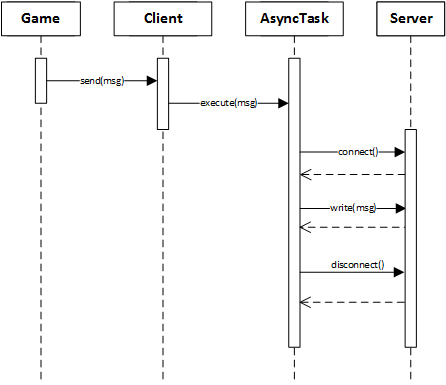
\includegraphics[width=\linewidth]{design/figures/tcp-client-sd.png}
\caption{Android TCP client sequence diagram.}
\end{figure}

The interface exposes the send function to the application to allow it to send data by internally using a class that extends AsyncTask.
\newpage
\subsubsection{TCP Message Structure}
\label{design:tcp-structure}
Due to this application leaking data by design, the message protocol does not require any encryption and can be relatively simple. There is only one type of message the application needs to send- data. The packet needs to include a uniquely identifiable value for the device that is running the game in order to track users. As it has relatively simple requirements the packet structure will be the packet type- in case of expansion-, device unique identifier followed by the payload. The fields will be delimited by a comma to allow the server to tokenize the packet for processing.

\subsection{TCP Server}
The TCP server will be incredibly simple as all that is required is the ability for clients to connect and post information to it. Due to this the server will be implemented in node.js as the LoC it takes to write a a TCP server to this standard is minimal.

\clearpage
\subsection{Requirements Matrix}
This section matches a given requirement from section \ref{requirements:specific} on page \pageref{requirements:specific} with proof that it has been considered in the design. 
\subsubsection{Honeypot Application}
\begin{table}[!h]
	\begin{center}
		\begin{tabular}{ | c |  p{12cm} | }
			\hline
			\textbf{Requirement} & \textbf{Verification} \\ \hline
			1 & The program flow in section \ref{program-flow} details how user defined options are required to create the interface.\\ \hline
			2 & Section \ref{parsing-probe} details how the SSID is captured and compared against the user defined value.\\ \hline
			3 & Capturing and parsing probe requests is detailed in section \ref{parsing-probe}. \\ \hline
			4 & Creating a fake access point is detailed in section \ref{design:create-ap}.\\ \hline
			5 & The TCP client is detailed in section \ref{hp-tcp}.\\ \hline
			6 & Section \ref{open-auth} looks at discovering vulnerable devices that are probing for open authentication networks. \\ \hline
			7 & Section unfinished.\\ 
			\hline
		\end{tabular}
	\end{center}
\end{table}

\subsubsection{Android Application}
\begin{table}[!h]
	\begin{center}
		\begin{tabular}{ | c |  p{12cm} | }
			\hline
			\textbf{Requirement} & \textbf{Verification} \\ \hline
			1 & Section \ref{design:flappy-bird} describes how the application will be a clone of a popular game.\\ \hline
			2 & The classes required for getting the GPS location are in section \ref{design:ag-lp-cd}.\\ \hline
			3 & Section unfinished\\ \hline
			4 & Sections \ref{design:ag-tcp-1} and \ref{design:tcp-structure} detail TCP client support. \\ 
			\hline
		\end{tabular}
	\end{center}
\end{table}

\subsubsection{Server Application}
\begin{table}[!h]
	\begin{center}
		\begin{tabular}{ | c |  p{12cm} | }
			\hline
			\textbf{Requirement} & \textbf{Verification} \\ \hline
			1 & Section unfinished.\\ \hline
			2 & Section unfinished.\\ 
			\hline
		\end{tabular}
	\end{center}
\end{table}
%%%%%%%%%%%%%%%%%%%%%%%%%%%%%%%%%%%%
\clearpage
\section{Implementation}
This section details the process taken to develop the various discrete components. The final implementation has been developed and tested in a controlled environment using a dedicated wireless network in order to meet the the required ethical standards.

\subsection{Operating System}
The laptop used to develop and run the application is running BackTrack 5 Revision 3 in a virtual machine on VirtualBox, on Windows 7.

\subsection{Ethernet Connection}
In order to bridge traffic and allow the compromised device to connect to the internet, the laptop must be attached via ethernet. In this case the laptop is connected to the wireless access point via an ethernet cable, and has it’s network adaptor set to bridged in the VirtualBox network settings.

\subsection{Setting up the Workstation}
The attackers laptop needs to be correctly wired to the network and setup in order to run the applications and perform the attack. A bash setup script was developed to quickly get the station ready to run the application:

\begin{verbatim}
#! \bin\bash
service ssh start
echo 1 > /proc/sys/net/ipv4/ip_forward
airmon-ng start wlan0
\end{verbatim}

This script enables SSH as the majority of development and testing was undertaken from my desktop PC, enables IP forwarding so we can bridge traffic from the fake access point to the wired network, and then starts a monitor interface from the wlan0 interface. Once this is complete the station is ready to run the honeypot application.
\clearpage
\subsection{Honeypot Application}
Figure \ref{hp-1} shows the Honeypot application running and outputting the probe requests of nearby devices. It's searching for a request from a device that is looking for the TESTAP network.

In this instance the Bucket server is not running, so probe requests are not being transmitted to the server.

\begin{figure}[h!]
\centering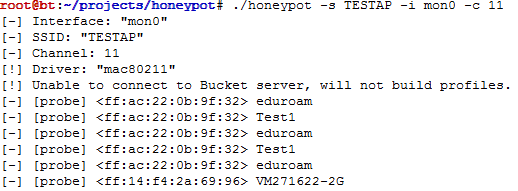
\includegraphics[width=\linewidth]{implementation/figures/hp-running-1.png}
\caption{Honeypot capturing probe requests.}
\label{hp-1}
\end{figure}

\subsubsection{Capturing Packets}
Using the Lorcon library we can parse captured packets, and decode them, by passing the lorcon loop function a callback. The callback passed to the lorcon loop takes a packet pointer parameter, which when called contains the captured frame. 

\begin{verbatim}
void packet_handler(lorcon_t *, lorcon_packet_t *, u_char *);
\end{verbatim}

To single out the frame type it is a case of indexing in the right location:

\begin{verbatim}
uint8_t packetType = packet->packet_header[HP_80211_TYPE];
\end{verbatim}

The lorcon library also offers a struct with extra info on 802.11 packets, which means the subtype could also be accessed as so:

\begin{verbatim}
struct lorcon_dot11_extra *extra;
extra = (struct lorcon_dot11_extra *)packet->extra_info;
\end{verbatim}

And then accessing the subtype field.

Once we have this information we can use a state style switch statement to determine where in the process of the association sequence we are, and react accordingly to incoming packets.

\subsubsection{Parsing Probe Requests}

Firstly the application needs to listen for probe request packets in order to get the SSIDs that nearby devices are searching for. To capture the SSID from the packet the application copies it from the header, using the SSID length field as an indexer:

\begin{verbatim}
for(i=0; i<packet->packet_header[HP_80211_P_SSID_LEN]; i++) {
	ssid[i] = packet->packet_header[HP_80211_P_SSID + i];
}
\end{verbatim}

This application is limited in that it only reacts to SSIDs in probe requests that match the SSID passed in as a command line argument. The filter is implemented in the parse probe request function and simply compares the SSID in the probe request to the SSID given, where ap info is a struct holding information about the virtual access point:

\begin{verbatim}
if(strcmp(ap_info.ssid, ssid) == 0) {
       ap_info.valid_probe = 1;
return 1;
}
\end{verbatim}

At this point, if a valid probe request has been found, the application pre-checks the authentication type of the AP that the device is probing for by sending a probe response and then parses the authentication response, checking whether the Authentication Algorithm is set to Open (i.e. 0). This check is performed so that a virtual access point is not created for devices that are probing for encrypted networks, as the application only handles unencrypted networks.

\subsubsection{Creating Probe Responses}

To create a probe response packet in lorcon we follow this process:

\begin{verbatim}
lcpf_proberesp(metapack, ap_info.dst_mac, ap_info.src_mac, ap_info.bssid, 
					0x00, 0x00, 0x00, ap_info.seq, 
					ap_info.timestamp, ap_info.beacon_int, ap_info.flags);
\end{verbatim}

The snippet above creates a probe request frame which then needs the required information element tags added, as determined through the research in section \ref{research:assoc-seq}:

\begin{verbatim}
lcpf_add_ie(metapack, IE_SSID_LEN, ap_info.ssid_len, ap_info.ssid);
lcpf_add_ie(metapack, IE_RATES, sizeof(rates)-1, rates);
lcpf_add_ie(metapack, IE_CHANNEL, 1, &channel);
lcpf_add_ie(metapack, IE_MISC, 1, "\x05");
lcpf_add_ie(metapack, IE_MISC, 1, "\x05");
txpacket = (lorcon_packet_t*)lorcon_packet_from_lcpa(context, metapack);
\end{verbatim}

\subsubsection{Creating a Fake Access Point}

When an open network has been discovered, the application forks and creates a virtual access point using airbase-ng and sends another probe response on behalf of the VAP to speed up the process of associating. 

\begin{verbatim}
.. snip..
childPID = fork();
	if(childPID >= 0) {
		if(childPID == 0) {
			// Child process
			snprintf(cmd, sizeof cmd, "airbase-ng --essid \%s -c \%i mon0",
				 ap_info.ssid, ap_info.channel);
			system(cmd);
.. snip..
\end{verbatim}

Figure \ref{client-connected} shows the application output when an access point is created and a client connects. In this instance the device has connected to the network WirelessLab.

\begin{figure}[h!]
\centering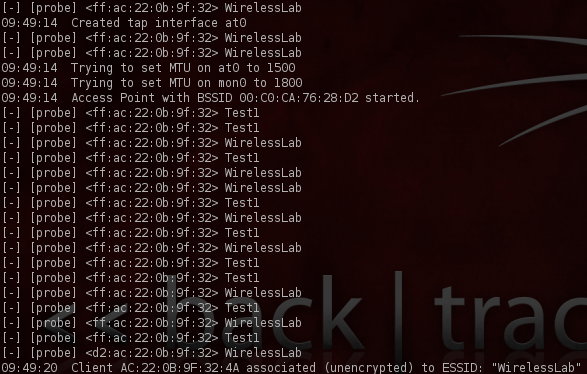
\includegraphics[width=\linewidth]{implementation/figures/client-assoc-1.png}
\caption{Virtual Access Point created and the client connecting.}
\label{client-connected}
\end{figure}

Once the application gets to this point it will no longer create virtual access points, as it is purposely limited to one, as defined in the requirements.

\subsubsection{Monitoring Data Packets}
As mentioned previously we need to bridge traffic from the tap interface created by airbase-ng to the wired interface that the Virtualbox host is on. To do this we perform the following steps:

\begin{verbatim}
brctl addbr wirelesslab-br
brctl addif wirelesslab-br eth0
brctl addif wirelesslab-br at0

ifconfig eth0 192.168.1.5 up
ifconfig at0 192.168.1.23 up

ifconfig wirelesslab-br 192.168.1.6 up
\end{verbatim}

This adds the two interfaces to the bridge created in the first command, then assigns an IP address to both of them. Once this step is complete traffic sent to the virtual access point will be forwarded across the eth0 interface and vice-versa.
\clearpage
 The filter required to get data packets in Wireshark travelling to the access point from the device is:

\begin{verbatim}
tcp && wlan.da == device_mac
\end{verbatim}

This then shows the tcp packets that have been forwarded across the bridge on to the wired network, and communicating with the server (192.168.1.5) on that network.

\begin{figure}[h!]
\centering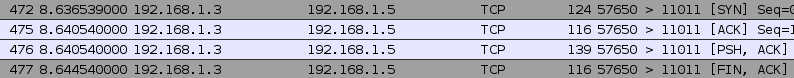
\includegraphics[width=\linewidth]{implementation/figures/wireshark captured.png}
\caption{Captured TCP packets from the device to the server.}
\end{figure}

The data found in the TCP packet is the location data that the app is relaying to the Bucket server:

\begin{figure}[h!]
\centering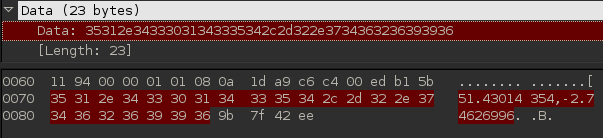
\includegraphics[width=\linewidth]{implementation/figures/wireshark-data.png}
\caption{Packet contents.}
\end{figure}

\newpage
\subsection{Leaky Game}
This application has been developed for Android and mimics the recently popular Flappy Bird style because of its simple nature, and possibility for exploiting the viral hype still surrounding it. It has been developed using Android Java and libgdx to handle the game functions and named Leaky Bird to reflect its actual purpose.

It was developed using the Eclipse IDE due to the support project creation support offered by libgdx tools, the process of which is detailed in a further section. The game was tested in a desktop environment to start with, before being deployed on a Nexus 7 for testing Android specific functionality.

\subsubsection{Project Structure}
Using the libgdx project setup tool removes the need for manually creating the projects and writing the boilerplate code required for the creation of cross-platform games. 

\begin{figure}[h!]
\centering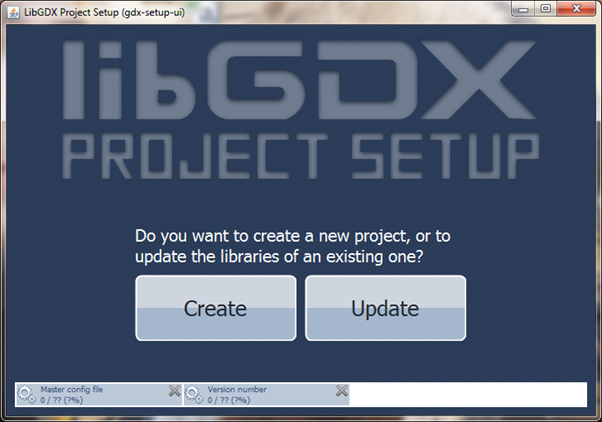
\includegraphics[width=\linewidth]{implementation/figures/gdx-setup-1.png}
\caption{libgdx setup tool.}
\end{figure}

It creates multiple Eclipse projects that link to one main project that holds the game code, thus effectively decoupling any platform specific code from the implementation. The projects created allow you to deploy on Android, desktop, web and iOS using robovm.
\clearpage
\begin{figure}[h!]
\centering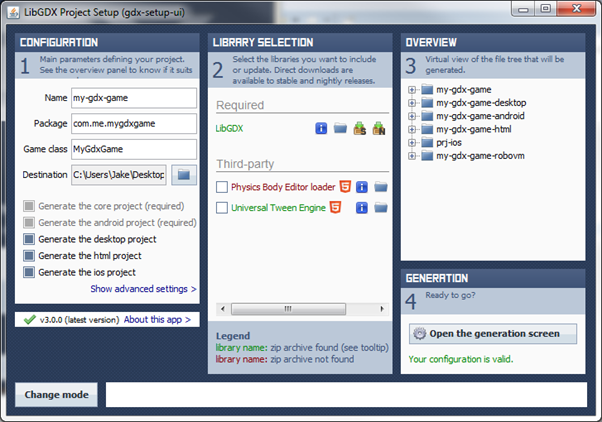
\includegraphics[width=\linewidth]{implementation/figures/gdx-setup-2.png}
\caption{Configuration screen.}
\end{figure}

Which when imported to Eclipse sets the workspace up automatically.

\begin{figure}[h!]
\centering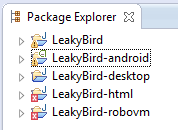
\includegraphics{implementation/figures/gdx-setup-3.png}
\caption{Eclipse project structure.}
\end{figure}
\clearpage
Whilst developing the game it was tested under the desktop deployment, and then when Android specific functions were required it was moved to testing on an actual device.

\subsubsection{Creating Interfaces}
As the Android application utilizes libgdx as it’s graphics library, we need to create a number of interfaces to allow it to use Android specific functions, for example GPS. The process in doing so is relatively straight forward. Firstly you need to create an interface to encapsulate the desired functions and then implement this interface in a class on the Android  side, and pass it through to the constructor of the game. 

In this project the interface takes the naming standard of XResolver, where X is the service it is handling, and the implementation takes the standard of PlatformX where Platform is the deployment platform, e.g. Android, desktop, etc., and X is the service.

If, for example, we were writing a resolver for adding two numbers, we would have an interface in the libgdx project as such:
\begin{verbatim}
public interface AdditionResolver {
    public int add(int a, int b);
}
\end{verbatim}
Then in the Android project implement the interface in a class:
\begin{verbatim}
public class AndroidAddition implements AdditionResolver {
    public AndroidAddition() {
    }

    @Override
    public int add(int a, int b) {
        return a + b;
    }
}
\end{verbatim}
And finally pass it through in the game initialiser in the Android MainActivity:
\begin{verbatim}
initialize(new LeakyBirdGame(androidAddition), cfg);
\end{verbatim}
Remembering to update the constructor of the Game class, then it is ready for use within the application while the game is running. In reality you wouldn’t need something as simple as an addition resolver, this is just to illustrate the steps to take.

\subsubsection{Getting the GPS Co-ordinates}
\label{getting-gps-coords}
The application has been developed to report the players location whilst they are playing the game. This required an interface to be written between Android Java and libgdx so that we could take advantage of Android's GPS support, as noted in the section prior to this about creating interfaces.

The two functions we need the libgdx side of the application to be able to access are the LocationManager class's getLatitude and getLongitude. The interface to pass to the LeakyBirdGame initialiser is:
\begin{verbatim}
public interface GpsResolver {
    public double getGPSLatitude();
    public double getGPSLongitude();
}
\end{verbatim}
It is named resolver due to libgdx being able to create desktop, HTML5 and iOS games from the same source code but with different entry points. Some of these entry points may not have GPS enabled so we have to be sure to wrap any calls to this class in a null check. On the Android side we can create a class, AndroidLocationProvider,  that implements this interface and allow the functions to wrap around the two LocationManager calls we need to make in order to get the coordinates. In the constructor of the class we need to get the name of the provider that our game will be using to get the location data, this can either be via GPS or network, the former being finer grained than the latter.
\begin{verbatim}
Criteria criteria = new Criteria();
provider = locationManager.getBestProvider(criteria, false);
\end{verbatim}
Where provider is a class level defined string and criteria is left intentionally default so the application will attempt to get the best provider available.

The two overridden interface functions require nearly identical implementations, with just the longitude/latitude selection switching between them:
\begin{verbatim}
 Location location = locationManager.getLastKnownLocation(provider);
 return location.getLatitude();
\end{verbatim}
As locationManager is passed through to the constructor from the Android MainActivity, it allows us to use a reference to it’s context internally to get the location data during the game’s execution.

In the libgdx project we can now access the GPS, assuming it has been passed through the constructor and named gpsResolver, through the two functions as so:
\begin{verbatim}
game.resolver.showToast(gpsResolver.getGPSLatitude());
\end{verbatim}
This is displayed using an Android Toast resolver that has been implemented in the same manner.

GPS co-ordinates can be changed in the Emulator, if not running on a device,  through the Dalvik Debug Monitor Service (DDMS) in Eclipse:
\begin{verbatim}
telnet localhost 5544 # Emulator port
geo fix  01.10 10.01
\end{verbatim}

\subsubsection{Android TCP Client}
This uses a similar process described in section \ref{getting-gps-coords} to access Android’s GPS functionality. Any network activity performed in an Android application must be done inside an AsyncTask rather than the UI thread, otherwise delayed activity may result in the application freezing. With this in mind another interface needed to be created to allow the wrapping of a class that extends AsyncTask, as this is in the Android library and inaccessible from libgdx.

The interface this time defines one function that must be implemented:
\begin{verbatim}
public boolean send(String msg);
\end{verbatim}

As the application is, by design, insecure and leaks data the function simply takes a string and sends it, using TCP, to the Bucket server. The message format for data packets is, as described in section \ref{design:tcp-structure}:
\begin{verbatim}
MESSAGE_ID,UNIQUE_ID,PAYLOAD
\end{verbatim}

The android implementation of this, AndroidTcpClient, consists of connection information class level variables and a private inner AsyncTask class that takes a string as a parameter for it’s DoInBackground function, and gives a boolean result, that takes care of the connecting and disconnecting to the server:

\begin{verbatim}
private class SenderTask extends AsyncTask<String, Void, String>
\end{verbatim}

Each time a message needs to be sent the AsyncTask connects to the TCP server and then, if successful, sends the message. This way should the server go down during testing, the application need not be restarted each time.
 
An interesting point to note is that for a period of time I could not get any output at the server end. The client application was connecting perfectly well and the server was displaying it’s connection information, but would not receive any data. This turned out to be because the send implementation was using a BufferedWriter and I had forgotten to add in:

\begin{verbatim}
out.flush();
out.close();
\end{verbatim}

after the write, which tells the BufferedWriter to send the data now rather than wait for it to be full.

Again the LeakyBirdGame constructor needs to be updated with the new parameter before it can be used in the game to send data.
\clearpage
\section{Conclusion}
\subsection{Defending Against Attacks}
Probe request frames are broadcast depending on what is in the preferred network list. This is what opens up smartphones to attack from such methods as undertaken in this project. Different mobile operating systems handle this list in different ways. For example, Android allows the user access to this list, and the ability to remove networks from it. Once removed from the list, the phone no longer broadcasts probe request frames for that SSID. iOS; however, does not allow access to this list and will broadcast frames for any previously connected SSID, unless the user disconnected from the network using the Forget This Network button available in the WiFi settings screen.

Proper management of this list would help the user to prevent this attack, or, at the very least, allow the user to make an informed decision about what network their phone is attempting to connect to. There a number of ways that you could implement this at application level. Being able to offer protection, or at the least information, at application level allows users with little knowledge to better protect themselves against malicious users. Ultimately, there is only so much you can do at this level, and all of the solutions require user interpretation.

One method would be to develop an application that ran as a service, storing information about each access point as the device connects to a network. The stored information would include the mac address of the access point that it has connected to, verified by the user, which would then allow the application to flag up any instances whereby the  device attempts to connect to a network with the same SSID where the mac address had changed.

This would work well on uniquely named IBSSs in a home setting, although it would become an issue if the device were to connect to a large ESS and were to roam between each AP. On each connection the user would have to verify the different mac address. The biggest issue this  is the simplicity in which a mac address can be spoofed. If the attacker were to be near the actual AP it would be trivial to find the real mac address and subsequently ensure any frames sent were from that address.

An extension on the previously detailed application would be to add geotagging to the stored access point information as it would allow the user to be notified when they are trying to connect to a network, for example, in Bristol that they usually do in Aberystwyth.

Overall the best course of action to take would be educating users on the importance of protecting their data, even that which they do not consider to be particularly sensitive can allow a foreign entity to profile and uniquely identify them. As we move towards advertisements as a means of sustaining internet businesses, and the consumer as the product business model (a la Facebook), it is imperative that we provide the necessary information to allow users to retain their privacy. 
\newpage
\subsection{Monitoring Probe Requests for Good}
\label{conclusion:for-good}
There are applications of this technique that can be used for non-malicious purposes, particularly in data analysis.

\subsection{Securing the Insecure}
\label{80211w}
It is widely acknowledged that cryptography can allow us to undo the damage that has been brought to light through the leaked documents because of the headache it causes surveillance agencies. Through-out this report I have alluded to new protocols and standard amendments that are being developed in response to the expanding usage of WiFi. 

The 802.11w amendment has recently been ratified and sets out to secure the management frames through adding cryptographic protection to deauthentication and disassociation frames to protect against spoofing; and a mechanism called Security Association Teardown Protection which protects association and authentication requests, through implementing a shared key authentication IE field called  Message Integrity Check. The MIC IE, whose structure is detailed in table \ref{tbl:mic}, includes fields for the key ID, IPN and most importantly, the Message Integrity Code which is the hash taken from the payload and MAC header of the management frame. 

\begin{table}[h!]
\begin{center}
	\begin{tabular}{|  p{2cm} |  p{2cm} | p{2cm} | p{2cm} | p{2cm} |}
		\hline
		ID & Length & Key ID & IPN & MIC\\ 
		\hline
	\end{tabular}
\end{center}
\caption{MIC IE field structure.}
\label{tbl:mic}
\end{table}

The key is generated using an EAPOL 4-way handshake between the station and the access point, meaning 802.11w can only be utilized if the network is using WPA/WPA2.

\subsection{Project Extensions}

Toward the end of writing this report a security research company unveiled their honeypot quadcopter device. This has the ability of being flown over a location, capturing devices, and bridging traffic back to a central server so that all traffic may be monitored by one application. This project is very well suited to fulfilling both the examples given that use this for good, but equally for bad. It should be noted; however, that the presence of a quadcopter is somewhat less inconspicuos than small devices planted around an area. 

During this project I also briefly touched upon porting this application to the Raspberry Pi due to not only its low price point, but Kali's support for ARM meant that doing so would be trivial. Further investigation in to solving the netlink library issue, either by fixing the outdated Lorcon configurator that checks for dependancies, or replacing with a native libpcap implementation would be required. Successfully doing this would open up a number of possibilities, from the quadcopter example detailed above, to coupling the Raspberry Pi with a GPS board to undertake some wardriving, or implementing any of projects for good mentioned in section \ref{conclusion:for-good}.
\newpage
\subsection{The End's Not Near; It's Here}
It has been a long process to get to the point where I currently am. When I started out deciding what type of Final Year Project I wanted to undertake, I knew I wanted to do something new, exciting, and geared more towards the academic side. Initially, after some research in to the Internet of Things, I decided that I would do a project on Wireless Sensor Networks titled ``Identification and Restoration of Compromised Nodes within a Wireless Sensor Network: A Remote Software-Based Attestation Approach'' as it was a developing area of interest. 

I wanted to understand how you could effectively detect malicious additions to software on a deployed node, and how you could then remotely repair the device. I spent a few months researching and learning about the Telos B motes and TinyOS, looking at existing protocols developed to perform code attestation, and ways to integrate remote updates of the delta between binaries in order to save power. It was around this point that I came across a paper, written not too long ago, that had set out to, and achieved, exactly what I had. With the- possibly naive- aim of producing a research paper from the project I took quite a knock and steered my project in a different direction.

Following the departure from 802.15.4 I took inspiration from the then developing stories of GCHQ and the NSA covertly monitoring people. To start with I stumbled upon the Evercookie and a recent paper on uniquely identifying users by fingerprinting data from browsers, such as screen size and available plug ins, and available fonts. I had decided that I would combine the two and create a framework for creating a unique identification number for a user, and store it on their computer in ways that circumvent cookie laws to show that there are other methods available to keep track of people. This project didn't hold my interest for too long, but did lead to me learning about an attack called HTTP Cache Poisoning. This attack, as I've mentioned in this report, allowed attackers to add bits of script on to the end of files without the user realising, thus offering a way to infect a users browser through only one contact on an open network.

As I looked in to HTTP Cache Poisoning more I realised I would need to extend my knowledge in the general area of network penetration testing and security. In doing so I gained an interest in other attacks that could be performed without the user realising, namely the honeypot attack.

I came in to this final project having no background knowledge of network security, penetration testing, or the 802.11 standard, only the parts I picked up during the research stages of the prior projects. As a result of this project I can now comfortably discuss various aspects relating to the security of Wifi networks and the inherent insecurities in the 802.11 standard. I’ve gained a solid understanding of network vulnerabilities, how to open gateways to attacks, and a number of attacks in different categories. Learning about the offensive side of security has certainly bolstered my knowledge of defending as well.

I feel the final iteration of my project has achieved the goals I set myself, namely: get a better understanding of how the monitoring of the general public is performed, how public entities such as GCHQ and the NSA implement these methods, and an improved insight in to just what pieces of information should actually be considered private.

In particular I am thrilled that I managed to get the Honeypot application running, capturing frames, and performing the association sequence programmatically. The expression of elation to see a device think that my application was an access point could be heard down the street; however, I was slightly disappointed that I ran into problems on the final step of the authentication sequence. No matter what I tried I could not get the correct flags set in the authentication response frame and have the device authenticate. I overcame this in the end by making use of existing software to handle the generation of a spoof access point, as this made it much easier to bridge traffic to the wired network, and most importantly allowed me to continue with my project.

Another issue I ran into was during the implementation of Leaky Bird. As it was my first attempt at writing a networked application for Android, although having general experience programming for Android, I was unaware of the need for all communications to be done in a class that extends AsyncTask. Couple this with the need to create interfaces for libgdx to access platform specific code and I was left with a number of development hours spent cursing at the Android Developer Tools IDE. After some research it became apparent that to beat the NetworkOnMainThreadException I needed to create a SenderTask class, inside the TcpClient class, that extends AsyncTask and ensure all connect, disconnect and send code is contained within it, as detailed in the implementation.

All in all I think this project has been incredibly beneficial in the ways mentioned above, but also in developing my writing skills by documenting to a high standard, and through learning LaTeX as a way of generating documents. Learning LaTeX was purely an academic decision, as the same style could be achieved through using Microsoft Word; however, I wanted to take the opportunity to add a new skill to my repertoire. 

As time goes on I would like to revisit both this project, and the initial project I set out to complete. Wireless network security is a field that I have become increasingly interested in during this past year, and putting the honeypot application on a Raspberry Pi, with a GPS/GSM shield, attaching it to a quadcopter, and flying it around sounds like too much of a fun opportunity to pass up.


\clearpage
\section{Appendix}
\subsection{Flappy Bird Spritesheet}
\begin{figure}[h!]
\centering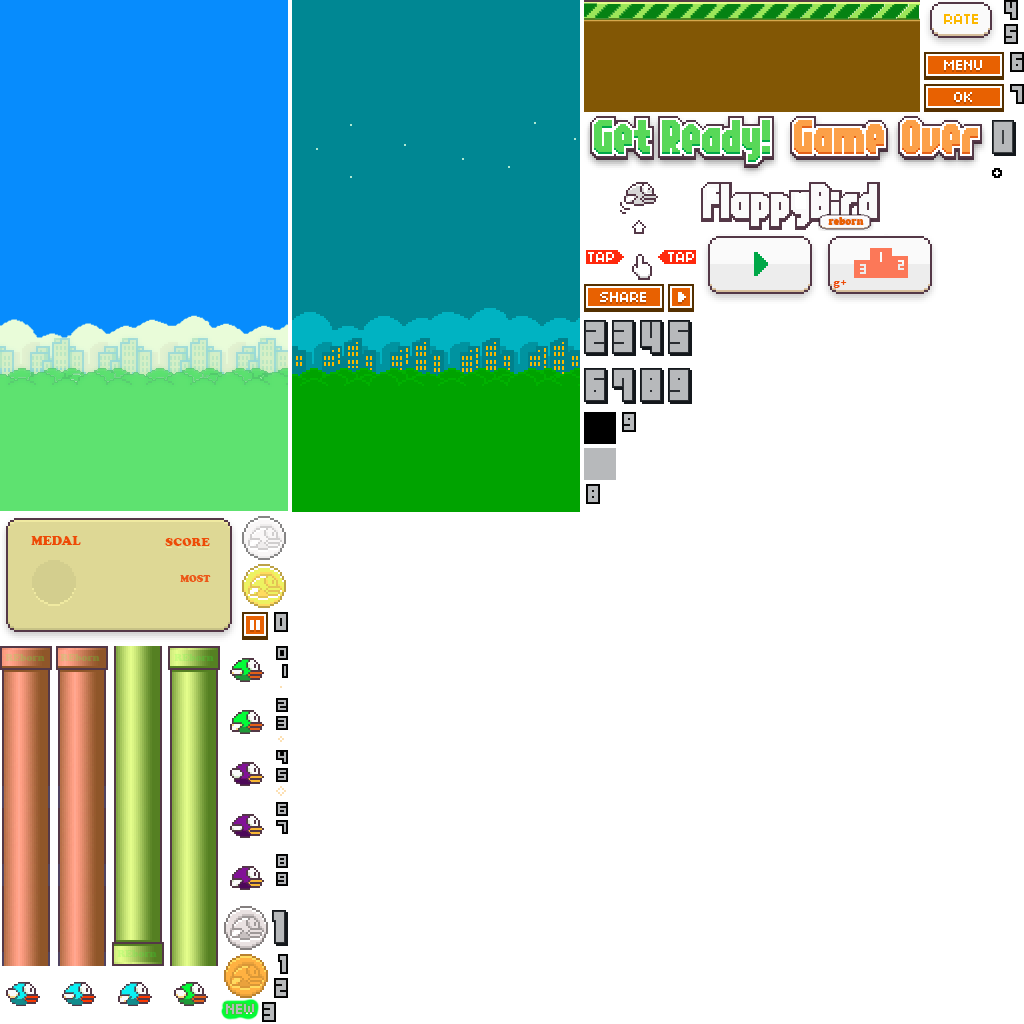
\includegraphics[width=\linewidth]{design/figures/leaky-spritesheet.png}
\caption{Flappy Bird spritesheet.}
\label{fig:leaky-spritesheet}
\end{figure}
\clearpage
% Bibtex dump
\printbibliography
% \cfoot{\thepage\ of \pageref{LastPage}}
\end{document}